% lint-skip: 未完成ステータス（figure/table caption 未対応，人手チェック時に解消予定）
\documentclass[../../main.tex]{subfiles}
\begin{document}

\begin{flushright}
  \footnotesize\textit{【自動文字起こし・要確認】}
\end{flushright}

{\bf [解答]} $0 < a < 1 \cdots \text{①}$ より，グラフは右図．$f(x) = \log(x-a)$ とする．

\begin{figure}[H]
  \centering
  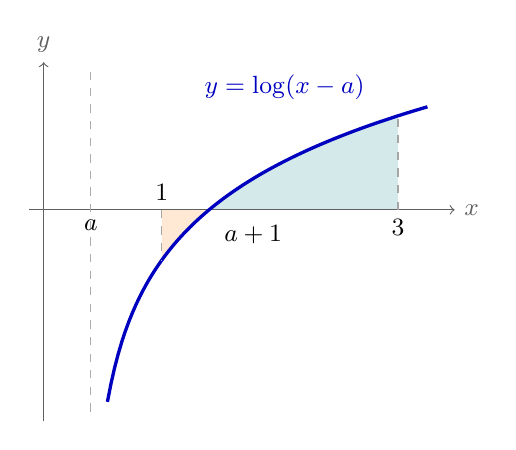
\begin{tikzpicture}[x=1.5cm,y=1.25cm,every node/.style={font=\small}]
    % a=0.4 の配置例．曲線は x=a+1 で x 軸を横切る．
    \fill[orange!17] (1,0)--plot[domain=1:1.4,samples=50]
    (\x,{ln(\x-0.4)})--cycle;
    \fill[teal!17] (1.4,0)--plot[domain=1.4:3,samples=80]
    (\x,{ln(\x-0.4)})--(3,0)--cycle;
    \draw[->,gray!75!black] (-0.12,0)--(3.48,0) node[right] {$x$};
    \draw[->,gray!75!black] (0,-2.15)--(0,1.50) node[above] {$y$};
    \draw[gray!65,dashed] (0.4,-2.05)--(0.4,1.4);
    \draw[blue!75!black,very thick,domain=0.54:3.25,samples=90]
    plot (\x,{ln(\x-0.4)});
    \draw[gray!70,dashed] (1,0)--(1,{ln(0.6)})
    (3,0)--(3,{ln(2.6)});
    \node[below] at (0.4,0) {$a$};
    \node[above] at (1,0) {$1$};
    \node[below right=2pt] at (1.4,0) {$a+1$};
    \node[below] at (3,0) {$3$};
    \node[blue!75!black,above left] at (2.8,1.02) {$y=\log(x-a)$};
  \end{tikzpicture}
  \caption{$x=1$から$x=3$までの曲線$y=\log(x-a)$と$x$軸で囲まれる部分}
\end{figure}

\paragraph{(1)}

\begin{align}
  \quad V(a) &= \int_1^3 \pi \{ f(x) \}^2 dx \\
  &= \pi \int_{1-a}^{3-a} (\log x)^2 dx \quad \cdots \text{②} \\
  &= \pi \left[ x(\log x)^2 - 2x(\log x - 1) \right]_{1-a}^{3-a} \\
  &= \pi \left\{ (3-a) \left\{ (\log(3-a))^2 - 2\log(3-a) + 2 \right\} - (1-a) \left\{ (\log(1-a))^2 - 2\log(1-a) + 2 \right\} \right\}
\end{align}

\paragraph{(2)}

②から
\begin{align}
  \dfrac{1}{\pi} V'(a) &= - (\log(3-a))^2 + (\log(1-a))^2 \\
  &= \{ \log(1-a) + \log(3-a) \} \{ \log(1-a) - \log(3-a) \} \\
  &= \log(1-a)(3-a) \cdot \log \dfrac{1-a}{3-a}
\end{align}

から，下表をうる．

\begin{center}
  \begin{table}[htb]
    \centering
    \begin{tabular}{|c|c|c|c|c|c|}
      \hline
      $a$ & $0$ & $\cdots$ & $2-\sqrt{2}$ & $\cdots$ & $1$ \\ \hline
      $V'$ & & $-$ & $0$ & $+$ & \\ \hline
      $V$ & & $\searrow$ & & $\nearrow$ & \\ \hline
    \end{tabular}
  \end{table}
\end{center}

\[
  \left(
    \begin{array}{l}
      (1-a)(3-a) \ge 1 \iff a \le 2-\sqrt{2}, 2+\sqrt{2} \le a \\
      \text{①から } \dfrac{1-a}{3-a} \le 1 \text{ である．}
  \end{array} \right)
\]

したがって，$a = 2-\sqrt{2}$ の時 $V$ は $\min$ で，この時，
\[
  \begin{cases}
    1-a = -1+\sqrt{2} \\
    3-a = 1+\sqrt{2}
  \end{cases}
\]
から $B = \log(-1+\sqrt{2}), A = \log(1+\sqrt{2})$ として，$B = -A$ だから
\begin{align}
  V(a) \cdot \dfrac{1}{\pi} &= (1+\sqrt{2}) \{ A^2 - 2A + 2 \} - (-1+\sqrt{2}) \{ B^2 - 2B + 2 \} \\
  &= (1+\sqrt{2}) \{ A^2 - 2A + 2 \} + (1-\sqrt{2}) \{ A^2 + 2A + 2 \} \\
  &= 2A^2 - 4\sqrt{2}A + 4
\end{align}
\[
  \therefore V(a) = 2\pi \left\{ (\log(1+\sqrt{2}))^2 - 2\sqrt{2}\log(1+\sqrt{2}) + 2 \right\}
\]

\end{document}
